% !Mode:: "TeX:UTF-8" 



\BiSection{2.5}{Figures}

\fancyhead[R]{本题2.5由鳌小mo不学无术完成}

对于图2.47的每个电路,画出$I_X$和晶体管跨导关于$V_X$的函数曲线草图,$V_X$从0变化到$V_{DD}$。在(a)中,假设$V_X$从变化到1.5V。

		\begin{figure}[H] %H为当前位置,!htb为忽略美学标准,htbp为浮动图形
	\begin{minipage}{\linewidth}
		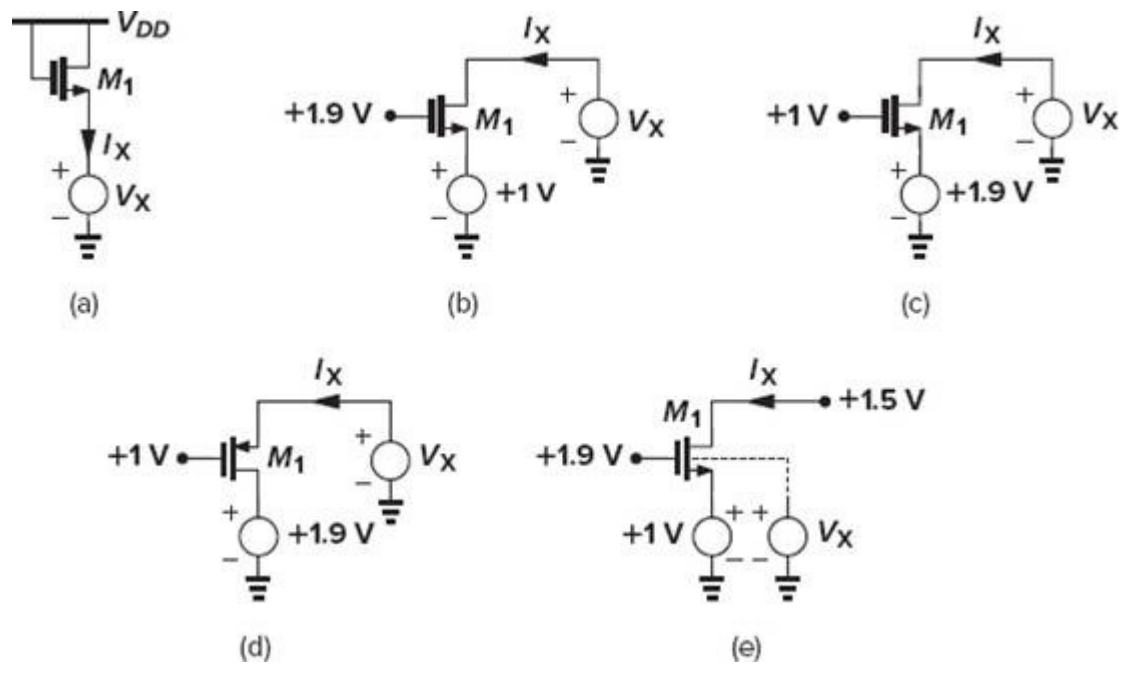
\includegraphics[width=1\linewidth]{2.5.47}
	\end{minipage}
	\caption*{图2.47} %最终文档中希望显示的图片标题
\end{figure}

解:

\scalebox{3}{(a)}

$V_{TH}=V_{TH0}+\gamma(\sqrt{|2\Phi_F+V_{SB}|}-\sqrt{|2\Phi_F|})=0.7+0.45(\sqrt{|0.9+V_{X}|}-\sqrt{|0.9|})$\textcolor{blue}{(公式见教材P20-2.23,参数$2\Phi_F$等见表2.1)}

$I_X=\frac{1}{2}\mu_nC_{ox}\frac{W}{L}(V_{GS}-V_{TH})^2(1+\lambda V_{DS})=\frac{1}{2}\mu_nC_{ox}\frac{W}{L}\{3-V_{X}-[0.7+0.45(\sqrt{|0.9+V_{X}|}-\sqrt{|0.9|})]\}^2[1+\lambda (3-V_{X})]=\frac{1}{2}\mu_nC_{ox}\frac{W}{L}(2.727-V_{X}-0.45\sqrt{0.9+V_{X}})^2[1.3-0.1V_X]$



\color{blue}{
	($I_X\text{随}V_{X}\text{的增大单调递减,}\lambda\text{见教材表2.1中}$)
	
}

\color{black}{
当$3-V_{X}-[0.7+0.45(\sqrt{|0.9+V_{X}|}-\sqrt{|0.9|})]>0\text{即}V_X<1.97V$时上式有效\textcolor{blue}{(否则NFET关)}

}

\color{blue}{
	\{
	
	\begin{figure}[H] %H为当前位置,!htb为忽略美学标准,htbp为浮动图形
		\begin{minipage}{\linewidth}
			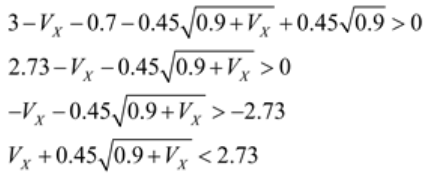
\includegraphics{2.5-1}
		\end{minipage}
	\end{figure}
	
	\begin{figure}[H] %H为当前位置,!htb为忽略美学标准,htbp为浮动图形
		\begin{minipage}{\linewidth}
			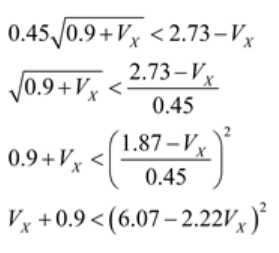
\includegraphics{2.5-2}
		\end{minipage}
	\end{figure}
	\begin{figure}[H] %H为当前位置,!htb为忽略美学标准,htbp为浮动图形
		\begin{minipage}{\linewidth}
			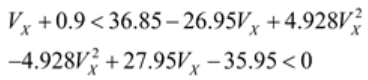
\includegraphics{2.5-3}
		\end{minipage}
	\end{figure}
	
	$V_{X}<1.97V\text{或}V_{X}>3.7V$
	
	$V_{X}<1.97V$($V_{DD}$最大值为3V)\textcolor{blue}{(见教材题目2.1上面那句话)}
	
	\}
	
	
}

\color{black}{
	$g_m=\sqrt{2\mu_nC_{ox}\frac{W}{L}I_D}=\sqrt{2\mu_nC_{ox}\frac{W}{L}I_X}$
	
	$=\sqrt{2\mu_nC_{ox}\frac{W}{L}\{\frac{1}{2}\mu_nC_{ox}\frac{W}{L}(2.727-V_{X}-0.45\sqrt{0.9+V_{X}})^2[1.3-0.1V_X]\}}=\mu_nC_{ox}\frac{W}{L}(2.727-V_{X}-0.45\sqrt{0.9+V_{X}})\sqrt{1.3-0.1V_X}$
	
	
		\begin{figure}[H] %H为当前位置,!htb为忽略美学标准,htbp为浮动图形
		\begin{minipage}{\linewidth}
			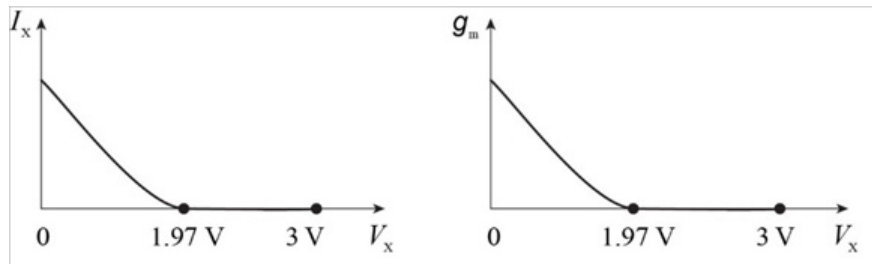
\includegraphics{2.5-4}
		\end{minipage}
		\caption*{图1} %最终文档中希望显示的图片标题
	\end{figure}
	
	\scalebox{3}{(b)}
	
	当$0<V_X<1V$时,NFET源漏交换,$I_X=\mu_nC_{ox}\frac{W}{L}[V_{OD}V_{DS}-\frac{1}{2}V_{DS}^2]=\mu_nC_{ox}\frac{W}{L}[(V_{GS}-V_{TH})V_{DS}-\frac{1}{2}V_{DS}^2]=\mu_nC_{ox}\frac{W}{L}[(1.9-V_X-0.7)(1-V_{X})-\frac{1}{2}(1-V_{X})^2]=-\frac{1}{2}\mu_nC_{ox}\frac{W}{L}(1-V_{X})(1.4-V_{X})$
	
	$g_m=\mu_nC_{ox}\frac{W}{L}V_{DS}=\mu_nC_{ox}\frac{W}{L}(1-V_{X})$\textcolor{blue}{($V_{DS}$不为常量不能用公式$g_m=\sqrt{2\mu_nC_{ox}\frac{W}{L}I_X}$,用P19的2.22,其由P13的2.8对$V_{GS}$求导得到)}
	
	当$V_X>1V$时,
	
	$V_{GS}-V_{TH}>V_{DS}$
	
	$1.9V-1V-0.7V>V_{X}-1$
	
	$V_X<1.2V$
	
	当$V_X<1.2V$时,NFET在线性区,$I_X=-\mu_nC_{ox}\frac{W}{L}[(V_{GS}-V_{TH})V_{DS}-\frac{1}{2}V_{DS}^2]=-\mu_nC_{ox}\frac{W}{L}[(1.9V-1V-0.7V)(V_{X}-1)-\frac{1}{2}(V_{X}-1)^2]$
	
	$g_m=\mu_nC_{ox}\frac{W}{L}V_{DS}=\mu_nC_{ox}\frac{W}{L}(V_{X}-1)$
	
	当$V_X>1.2V$时,NFET在饱和区,$I_X=\frac{1}{2}\mu_nC_{ox}\frac{W}{L}(V_{GS}-V_{TH})^2=\frac{1}{2}\mu_nC_{ox}\frac{W}{L}(1.9V-1V-0.7V)^2=\frac{1}{2}\mu_nC_{ox}\frac{W}{L}(0.2V)^2$
	
	$g_m=\sqrt{2\mu_nC_{ox}\frac{W}{L}I_X}=\sqrt{2\mu_nC_{ox}\frac{W}{L}[\frac{1}{2}\mu_nC_{ox}\frac{W}{L}(0.2V)^2]}=0.2\mu_nC_{ox}\frac{W}{L}$
	
			\begin{figure}[H] %H为当前位置,!htb为忽略美学标准,htbp为浮动图形
		\begin{minipage}{\linewidth}
			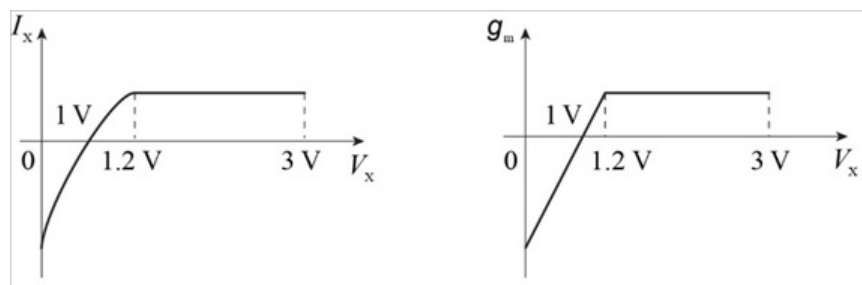
\includegraphics{2.5-5}
		\end{minipage}
		\caption*{图2} %最终文档中希望显示的图片标题
	\end{figure}
	
	\scalebox{3}{(c)}
	
	$V_{GS}>V_{TH}$
	
	$1V-V_{X}>0.7V$
	
	$V_{X}<0.3V$
	
	当$V_X>0.3V$时,NFET关
	
	$V_{GS}-V_{TH}=1V-V_{X}-0.7V=0.3V-V_{X}$
	
	$V_{DS}=1.9V-V_{X}$
	
	当$V_X<0.3V$时,NFET在饱和区,$I_X=-\frac{1}{2}\mu_nC_{ox}\frac{W}{L}(V_{GS}-V_{TH})^2=-\frac{1}{2}\mu_nC_{ox}\frac{W}{L}(0.3V-V_{X})^2$
	
	$g_m=\frac{2I_X}{V_{GS}-V_{TH}}=-\mu_nC_{ox}\frac{W}{L}(0.3V-V_{X})$\textcolor{blue}{(根号非负不能用$g_m=\sqrt{2\mu_nC_{ox}\frac{W}{L}I_X}=\sqrt{2\mu_nC_{ox}\frac{W}{L}[-\frac{1}{2}\mu_nC_{ox}\frac{W}{L}(0.3V-V_{X})^2]}$,用P18的2.20)}
	
				\begin{figure}[H] %H为当前位置,!htb为忽略美学标准,htbp为浮动图形
		\begin{minipage}{\linewidth}
			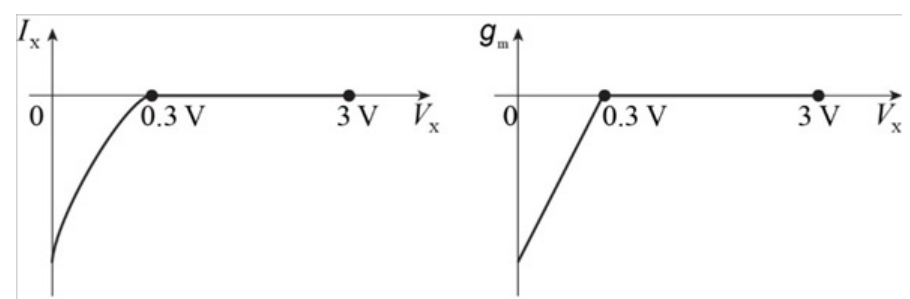
\includegraphics{2.5-6}
		\end{minipage}
		\caption*{图3} %最终文档中希望显示的图片标题
	\end{figure}
	
	\scalebox{3}{(d)}
	
	$V_{GS}+|V_{TH0}|=-0.9V+|-0.8V|=-0.1V$
	
	$V_{DS}=V_{X}-1.9V$
	
	当$V_{GS}+|V_{TH0}|>V_{DS}\text{即}V_X<1.8V$时,PFET在饱和区,$I_X=-\frac{1}{2}\mu_pC_{ox}\frac{W}{L}(V_{GS}-V_{TH0})^2=-\frac{1}{2}\mu_pC_{ox}\frac{W}{L}(-0.9-(-0.8))^2=-\frac{1}{2}\mu_pC_{ox}\frac{W}{L}(0.1)^2$
	
	$g_m=\frac{2I_X}{V_{GS}-V_{TH}}=-0.1\mu_pC_{ox}\frac{W}{L}$
	
	当$1.8V<V_X<1.9V$时,PFET在线性区,$I_X=-\mu_pC_{ox}\frac{W}{L}[(V_{GS}-V_{TH})V_{DS}-\frac{1}{2}V_{DS}^2]=-\mu_pC_{ox}\frac{W}{L}[(-0.9-(-0.8))(V_{X}-1.9)-\frac{1}{2}(V_{X}-1.9)^2]$
	
	$g_m=\mu_pC_{ox}\frac{W}{L}V_{DS}=\mu_pC_{ox}\frac{W}{L}(V_{X}-1.9)$
	
	当$V_X>1.9V$时,PFET源漏交换,$I_X=\mu_pC_{ox}\frac{W}{L}[(V_{GS}-V_{TH})V_{DS}-\frac{1}{2}V_{DS}^2]=\mu_pC_{ox}\frac{W}{L}[(1-V_{X}-(-0.8))(1.9-V_{X})-\frac{1}{2}(1.9-V_{X})^2]$
	
	$g_m=\mu_pC_{ox}\frac{W}{L}V_{DS}=\mu_pC_{ox}\frac{W}{L}(1.9-V_{X})$
	
					\begin{figure}[H] %H为当前位置,!htb为忽略美学标准,htbp为浮动图形
		\begin{minipage}{\linewidth}
			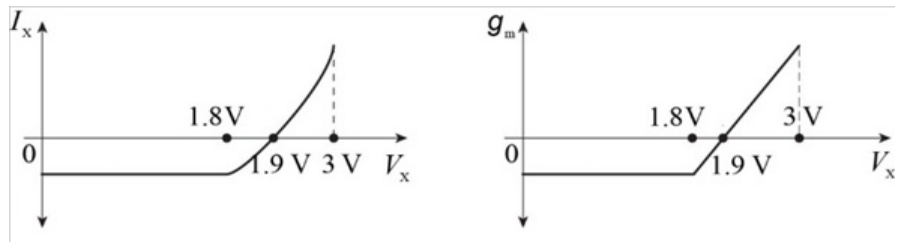
\includegraphics{2.5-7}
		\end{minipage}
		\caption*{图4} %最终文档中希望显示的图片标题
	\end{figure}
	
	\scalebox{3}{(e)}
	
	$V_{TH}=V_{TH0}+\gamma(\sqrt{|2\Phi_F+V_{SB}|}-\sqrt{|2\Phi_F|})=0.7+0.45(\sqrt{|0.9+1-V_{X}|}-\sqrt{|0.9|})=0.7+0.45(\sqrt{1.9-V_{X}}-\sqrt{0.9})$\textcolor{blue}{(公式见教材P20-2.23,参数$2\Phi_F$等见表2.1)}
	
	$I_X=\frac{1}{2}\mu_nC_{ox}\frac{W}{L}(V_{GS}-V_{TH})^2=\frac{1}{2}\mu_nC_{ox}\frac{W}{L}\{0.9-[0.7+0.45(\sqrt{1.9-V_{X}}-\sqrt{0.9})]\}^2=\frac{1}{2}\mu_nC_{ox}\frac{W}{L}[0.2-0.45(\sqrt{1.9-V_{X}}-\sqrt{0.9})]^2$
	
	$g_m=\sqrt{2\mu_nC_{ox}\frac{W}{L}\{\frac{1}{2}\mu_nC_{ox}\frac{W}{L}[0.2-0.45(\sqrt{1.9-V_{X}}-\sqrt{0.9})]^2\}}=\mu_nC_{ox}\frac{W}{L}[0.2-0.45(\sqrt{1.9-V_{X}}-\sqrt{0.9})]$
	
	当$V_{BS}$不为常量时,NFET在线性区的$g_m=\mu_nC_{ox}\frac{W}{L}V_{DS}=0.5\mu_nC_{ox}\frac{W}{L}$
	
	对比以上二式
	
						\begin{figure}[H] %H为当前位置,!htb为忽略美学标准,htbp为浮动图形
		\begin{minipage}{\linewidth}
			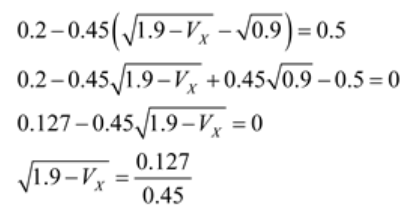
\includegraphics{2.5-8}
		\end{minipage}
	\end{figure}
	
						\begin{figure}[H] %H为当前位置,!htb为忽略美学标准,htbp为浮动图形
		\begin{minipage}{\linewidth}
			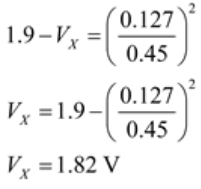
\includegraphics{2.5-9}
		\end{minipage}
	\end{figure}
	
	当$1.82V<V_X$时,NFET在线性区,$I_X=\mu_nC_{ox}\frac{W}{L}[(V_{GS}-V_{TH})V_{DS}-\frac{1}{2}V_{DS}^2]=\mu_nC_{ox}\frac{W}{L}\{[0.9-0.7-0.45(\sqrt{1.9-V_{X}}-\sqrt{0.9})](0.5)-\frac{1}{2}(0.5)^2\}$
	
							\begin{figure}[H] %H为当前位置,!htb为忽略美学标准,htbp为浮动图形
		\begin{minipage}{\linewidth}
			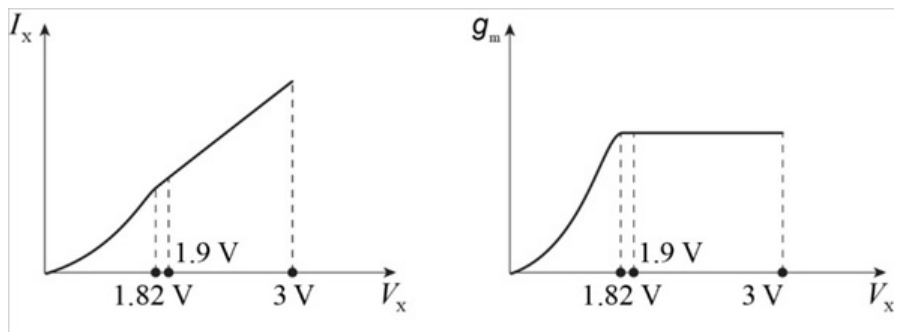
\includegraphics{2.5-10}
		\end{minipage}
		\caption*{图5} %最终文档中希望显示的图片标题
	\end{figure}
	

	
}

